\section{Our Experiment}
\subsection{Infrastructure}
\paragraph{}As the experiment's infrastructure we will describe the frameworks used during the implementation.
\subsubsection{Apache Spark}
The last decade, analyzing big data is at its peek. Lots of data are produced on daily basis. This means that the need of extracting information from them is raised. 
Lots of techniques has been used. The most common technique to do this in a distributed way is map-reduce.

Spark's predecessor, hadoop map reduce, was for a long time at its peak.
 Hadoop map reduce, is a distributed map-reduce system, 
this means that it has a mechanism to distribute work on nodes 
and a common interface for handling data. In hadoop's case this was able
 to happen due to Apache hadoop yarn and the HDFS (hadoop distributed file system).
 When a job was scheduled, data were loaded by the hdfs to a worker, 
then the worker was putting the result back to the hdfs. 
Map-reduce is a method that is around a lot time for handling large amounts of data. 
It has two basic processes, Map which is responsible for turning the data into key value pairs, and Reduce which takes those pairs and turns them into valuable data.

As mentioned in \cite{ibmMapReduce:5}, "The term MapReduce actually refers to two separate and distinct tasks that Hadoop programs perform. The first is the map job, which takes a set of data and converts it into another set of data, where individual elements are broken down into tuples (key/value pairs). The reduce job takes the output from a map as input and combines those data tuples into a smaller set of tuples. As the sequence of the name MapReduce implies, the reduce job is always performed after the map job."


If we would like to see where in the DIKW (Data Information Knowledge Wisdom) stack those processes belong, the map would start with data and the reduce will end up with information.



\begin{figure}[h]
	\centering
	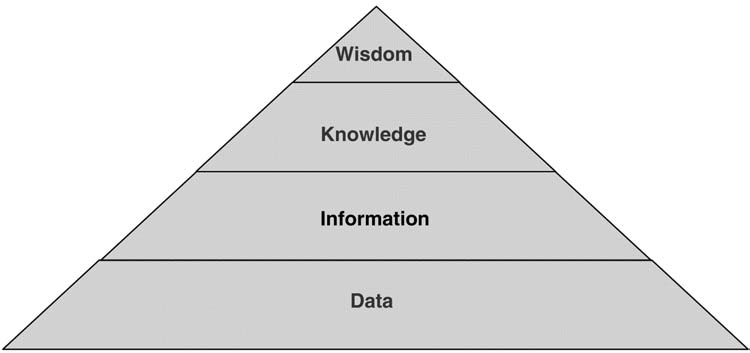
\includegraphics[width=0.5\textwidth]{images/DIKW.png}
	\caption{\bfseries Data Information Knowledge Wisdom Pyramid \cite{TheWisdomHierachy:7}}
	\label{dikw}
\end{figure}

Hadoop was the core map-reduce framework the last years.
As it is described in \cite{Hadoop:9}, and shown in the figure \ref{hadoopStack} hadoop uses hadoop yarn in order to coordinate which process will run on which machine. Also it uses the HDFS (Hadoop Distributed File System) in order to have a common reference for the files over the network. Last but not least, hadoop ecosystem is supported by the Hadoop Commons library. 

\begin{figure}[h]
	\centering
	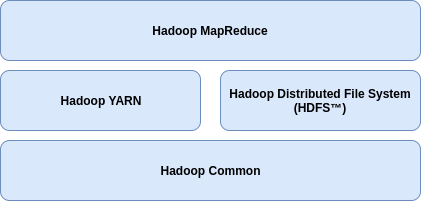
\includegraphics[width=0.5\textwidth]{images/hadoop-stack.png}
	\caption{\bfseries Hadoup Software Stack}
	\label{hadoopStack}
\end{figure}

 In 2009 UC Berkley developed spark \cite{DatabricsSpark:8}.
Spark's predecessor, hadoop map reduce, was for a long time at its peak. Hadoop map reduce, is a distributed map-reduce system, this means that it has a mechanism to distribute work on nodes and a common interface for handling data. In hadoop's case this was able to happen due to Apache hadoop yarn and the HDFS (hadoop distributed file system). When a job was scheduled, data were loaded by the hdfs to a worker, then the worker was putting the result back to the hdfs. 

\paragraph{}Apache spark is the new trend on distributed computation and map-reduce. 
But first things first, what is map-reduce? \\
apache mesos -> data center operating system, references
\\
But innovation knocked the door and resilient distributed datasets entered the room. In spark world, data are loaded to hdfs as before. Then spark loads them in an RDD, this means that data are now accessible on each machine's memory. Any transformation done to a RDD results a RDD, and so forth. After all the transformations are done, spark can transform the results to a file in hdfs.

\begin{figure}[ht]
  \centering
    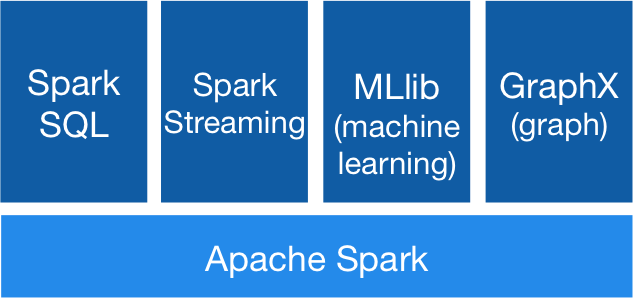
\includegraphics[width=0.5\textwidth]{images/spark-stack.png}
    \caption{\bfseries Apache spark stack \cite{ApacheSpark:1}}
   \label{apacheSparkStack}
\end{figure}

How spark differentiates from its predecessors\\
Spark lightweight in memory data transformation 
Resilient Distributed Datasets (RDDs) \\
mllibs\\
add spark jira note \\\\
Important note: mention als distributed broadcasting implementation. 
\\\\
When a RDD is been broadcasted in Apache Spark, this RDD becomes a local matrix to each machine. This means that you can use it for local calculations. This adds an overload to each machine depending on RDD's size. But it eliminates the network usage.
//cite the mastering apache spark book
\cite{ApacheSpark:1} \\
a Spark cluster to be created on AWS EC2 storage.\\
New trends on spark https://github.com/apache-spark-on-k8s/spark cite this repository too.
\subsection{Dataset}
What is the dataset about. This dataset contains users, movies and the rating user made about the movies.
This dataset is splited to multiple subsets of 80000 training sets and respective 20000 reviews.
This dataset has been used by the related work on .....
\cite{MovieLens:3}

\subsection{Implementation and assumptions}
During the implementation I had to make some assumptions and choices. The first of choices was the framework and the programming language that the implementation would take place. The framework that has been chosen, as you may had already figured out, is apache spark due to its trend and the high scalability it offers. The language of choice was scala, due to its functional nature.
\subsection{Metrics}
After the implementation I had to make the choice of the metrics I was going to use.
\subsubsection{Mean Absolute Error}
As metrics are commonly used the MSE, RMSE and MAE. Due to the fact that the author prefers the last one, MAE was used in this experiment.
\begin{equation}
MAE = \frac{\sum_{i=1}^{n}{|y_{i}-x_{i}|} }{n} = \frac{\sum_{i=1}^{n}\sqrt{{(y_{i}-x_{i})}^{2}}}{n}
\end{equation}
\subsubsection{Execution Time}
Time is measured in milliseconds.
Execution time is always a measure when we are comparing algorithms. 
Even more if those algorithms execution time is heavily dependent to their complexity and not their resources.
